\documentclass[a4paper,14pt]{extreport}
	\usepackage[left=1.5cm,right=1.5cm,
	    top=1.5cm,bottom=2cm,bindingoffset=0cm]{geometry}
	\usepackage{scrextend}
	\usepackage[T1,T2A]{fontenc}
	\usepackage[utf8]{inputenc}
	\usepackage[english,russian,ukrainian]{babel}
	\usepackage{tabularx}
	\linespread{1.3}
	\usepackage{amssymb}
	\usepackage{fp}
	\usepackage{color}
	\usepackage{amsmath}
	\usepackage{mathrsfs}
	\usepackage{listings}
	\usepackage{graphicx}
	\graphicspath{ {./images/} }
	\usepackage{lipsum}
	\usepackage{xcolor}
	\usepackage{multirow}
	%\usepackage[table,xcdraw]{xcolor}
	\usepackage{hyperref}
	\usepackage{tcolorbox}
	\usepackage{tikz}
	\usepackage[framemethod=TikZ]{mdframed}
	\usepackage{wrapfig,boxedminipage,lipsum}
	\usepackage{tcolorbox}



\begin{document}
\newtcbox{\xmybox}[1][red]{on line, arc=7pt,colback=#1!10!white,colframe=#1!50!black, before upper={\rule[-3pt]{0pt}{10pt}},boxrule=1pt, boxsep=0pt,left=6pt,right=6pt,top=2pt,bottom=2pt}

\begin{titlepage}
	\begin{center}
	\large
	Національний технічний університет України \\ "Київський політехнічний інститут імені Ігоря Сікорського"


	Факультет Електроніки

	Кафедра мікроелектроніки
	\vfill

	\textsc{ЗВІТ}\\

	{\Large Про виконання лабораторної роботи №4\\
	з дисципліни: «Функціональна електроніка»\\[1cm]

	Енергонезалежна пам'ять


	}
	\bigskip
	\end{center}
	\vfill

	\newlength{\ML}
	\settowidth{\ML}{«\underline{\hspace{0.4cm}}» \underline{\hspace{2cm}}}
	\hfill
	\begin{minipage}{1\textwidth}
	Виконавець:\\
	Студент 4-го курсу \hspace{4cm} $\underset{\text{(підпис)}}{\underline{\hspace{0.2\textwidth}}}$  \hspace{1cm}А.\,С.~Мнацаканов\\


	Перевірила: \hspace{5.9cm} $\underset{\text{(підпис)}}{\underline{\hspace{0.2\textwidth}}}$  \hspace{1cm}Т.\,Ю.~Обухова\\

	\end{minipage}

	\vfill

	\begin{center}
	2021
	\end{center}
\end{titlepage}






\textbf{Мета роботи} -- ознайомлення з фізичними принципами, архітектурою та
алгоритмами запису/зчитування/стирання енергонезалежної пам’яті
EEPROM та Flash
\begin{center}
\textbf{Порядок виконання роботи}
\end{center}
	\begin{enumerate}


	\item  Зібрати стенд. При вимкненому живленні підключити джерела 5 В та
14 В, генератор та осцилограф до відповідних роз’ємів основного модуля.
	\item  Встановити змінний модуль EEPROM-пам’яті. Ввімкнути живлення.
	\item  Відповідно до додатку 2 провести процедуру повного стирання
інформації з мікросхеми.
	\item  Відповідно до додатку 2 провести процедуру запису байту інформації у
задану викладачем комірку пам’яті мікросхеми. В якості байту даних
береться довільне число в діапазоні від 0 до 255 у двійковій системі.
	\item  Відповідно до додатку 2 провести процедуру зчитування інформації з
попередньо записаної комірки пам’яті мікросхеми. Необхідно врахувати, що
для коректного зчитування даних перемикачі на панелі 3 повинні бути
виключені.
	\item  Переключити перемикач 11 у положення роботи від генератора.
Перевести всі перемикачі і кнопки у положення що відповідають алгоритму
зчитування EEPROM-пам’яті (див. додаток 2). Зняти осцилограми
зчитування біту даних.
	\item  Переключити перемикач 11 у положення роботи від кнопки. Вимкнути
живлення основного модуля стенда. Відключити блок живлення 12 В.
Встановити змінний модуль Flash-пам’яті. Ввімкнути живлення.
	\item  Відповідно до додатку 3 провести процедуру повного стирання
інформації з мікросхеми.
	\item  Відповідно до додатку 3 провести процедуру запису байту інформації у
задану викладачем комірку пам’яті мікросхеми. В якості байту даних
береться довільне число в діапазоні від 0 до 255 у двійковій системі.
	\item  Відповідно до додатку 3 провести процедуру зчитування інформації з
попередньо записаної комірки пам’яті мікросхеми. Необхідно врахувати, що
для коректного зчитування даних перемикачі на панелі 3 повинні бути
виключені.
	\item  Переключити перемикач 11 у положення роботи від генератора.
Перевести всі перемикачі і кнопки у положення що відповідають алгоритму
зчитування Flash-пам’яті (див. додаток 3). Зняти осцилограми зчитування
біту даних.
	\item  Переключити перемикач 11 у положення роботи від кнопки.
Вимкнути живлення основного модуля стенда.
	\end{enumerate}

\begin{figure}[h!]
	\center{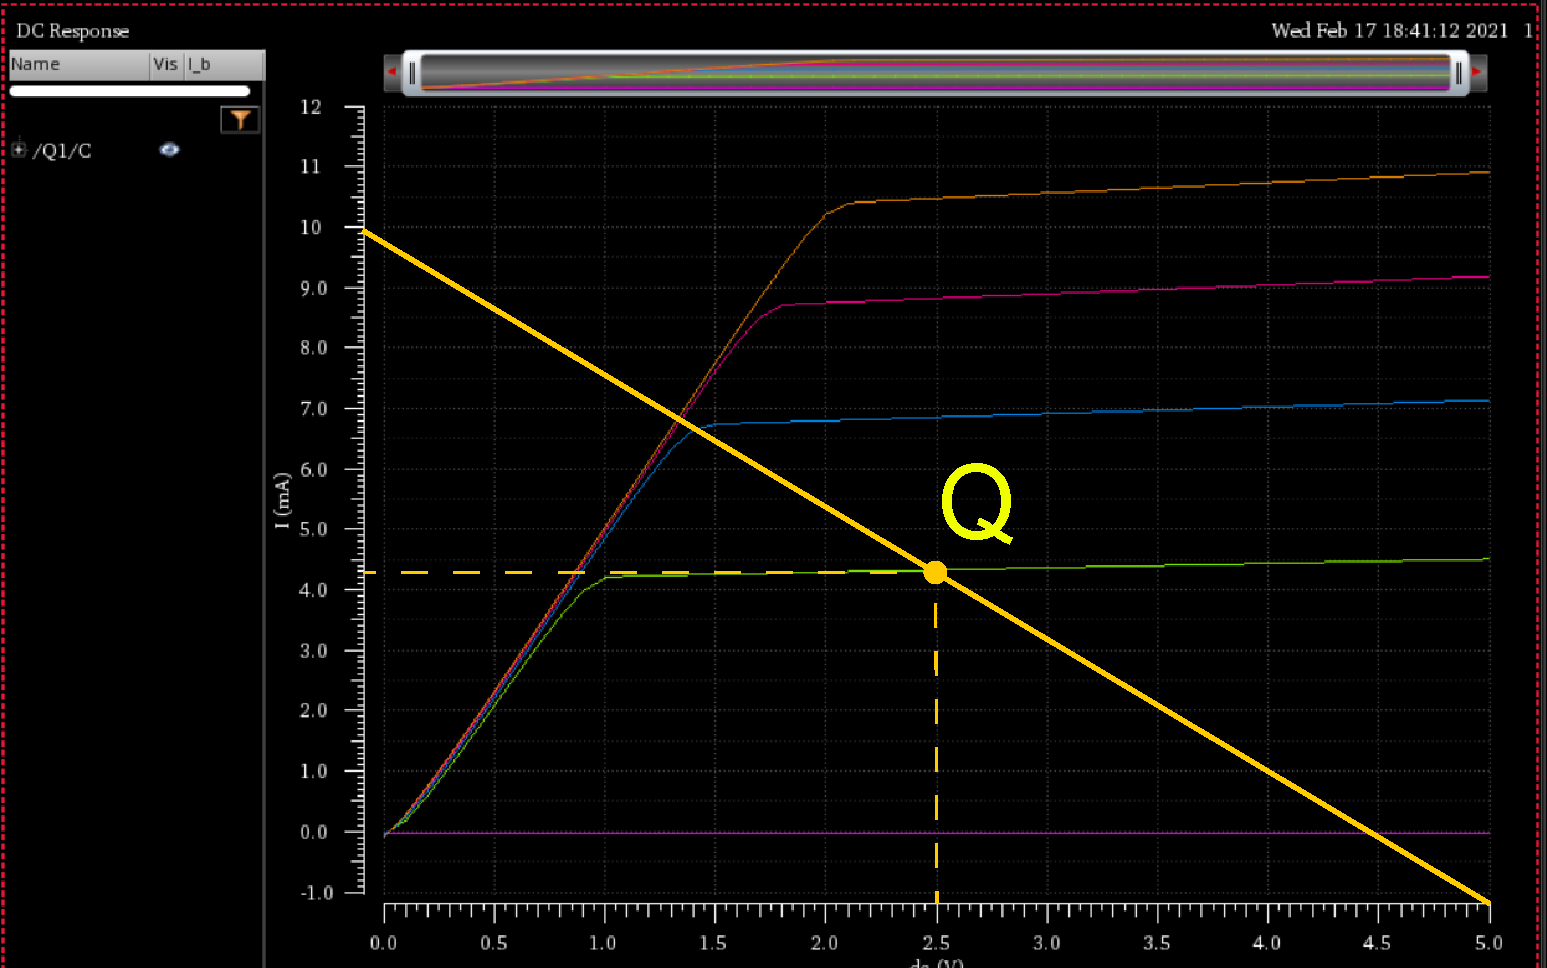
\includegraphics[width=0.6\linewidth]{1.jpg}}
	%\caption{Принципова схема для логічної функції «АБО» на тунельному діоді.}
	\label{ris1}
\end{figure}

\newpage

\begin{center}
\textbf{Обробка результатів}
\end{center}
Алгоритм запису в EEPROM-пам’ять:\\ 

\begin{enumerate}
\item Алгоритм запису в EEPROM-пам’ять:
\item Подати напругу 12 В на вивід ОЕ/Vpp  і напруги живлення 5 В на вивід Vcc. 
\item Виставити необхідну адресу за допомогою адресних перемикачів № 1-16.
\item Виставити необхідний байт перемикачами вводу/виводу даних № 1-8.
\item Подати V0 на вивід СЕ.
\end{enumerate}

Алгоритм запису в FLASH-пам’ять: \\ 

\begin{enumerate}
\item Завантаження трьох байт для «Захисту програмних даних». Адреса встановлюється за допомогою перемикачів № 1-16, дані - №1-8. Запис відбувається натиском кнопки «9»\\
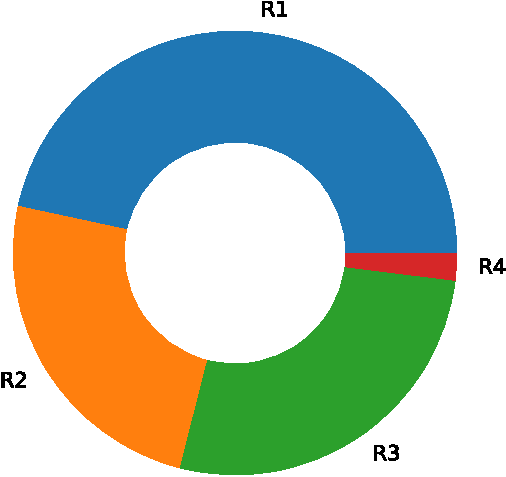
\includegraphics[width=0.5\linewidth]{2.png}
\item Подати напругу живлення 5В на VDD, на OE -V1 і на СЕ/WE - V0.

\item Завантажити дані користувача. Встановлення адреси, даних і запис відбувається аналогічно до пункту.

\end{enumerate}


 \begin{table}[h!]
\begin{tabular}{c|c|c}
\multirow{3}{*}{ комірка}  & 51  & 11001    \\
                  & 101 & 1100101  \\
                  & 151 & 10010111 \\ \hline
\multirow{3}{*}{ число} & 22  & 10110    \\
                  & 66  & 1000010  \\
                  & 44  & 101100  
\end{tabular}
\end{table}




\vspace*{1cm}
Висновок:  в ході даної лабораторної роботи було вивчено фізичні принципи, архітектура та алгоритми запису/зчитування/стирання енергонезалежної пам’яті EEPROM та Flash. Для EEPROM-памяті процедура запису – єдиний спосіб змінити значення у комірці з «1» на «0». FLASH-память реалізуються за допомогою певних послідовностей команд, кожна з яких має свою адресу для запису, проте перед тим як записати у сектор байт, цей сектор необхідно повністю стерти. Під час цього процесу, будь-які інші команди ігноруються.







\end{document}